% Generated from archived contact-error endpoint reports; three repeats, sample SD.
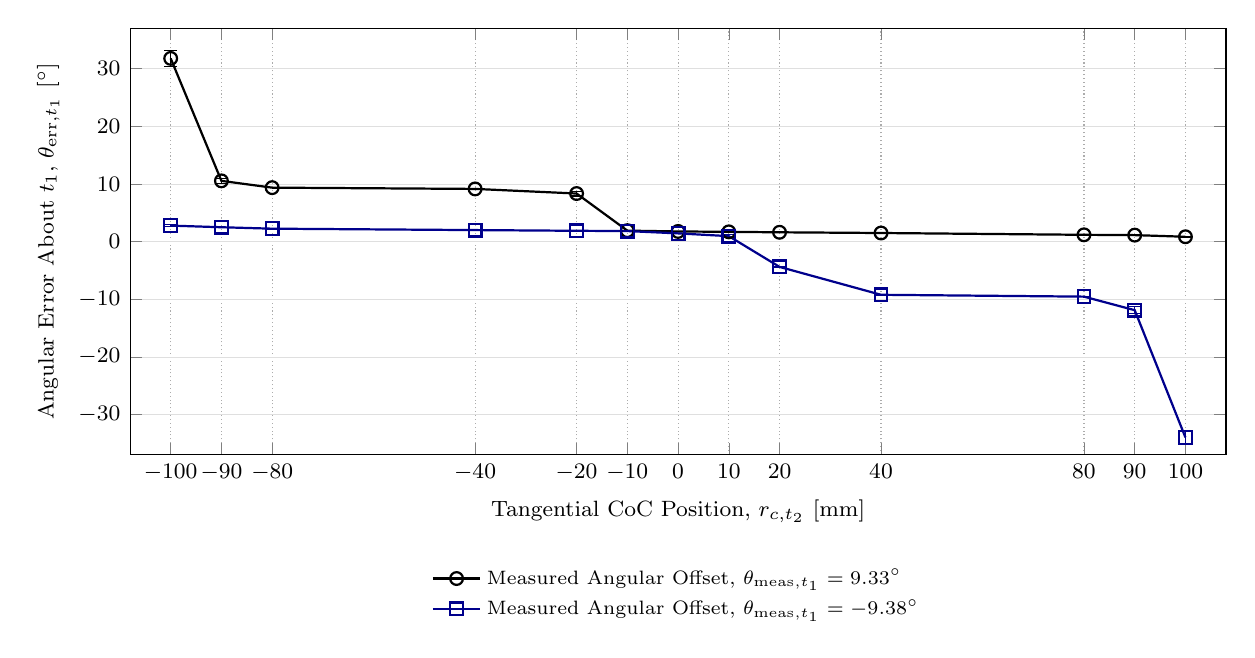
\begin{tikzpicture}
\begin{axis}[
    width=15.5cm, height=7.0cm,
    xmin=-108, xmax=108, ymin=-37, ymax=37,
    xtick={-100,-90,-80,-40,-20,-10,0,10,20,40,80,90,100}, ytick={-30,-20,-10,0,10,20,30},
    xlabel={Tangential CoC Position, \(r_{c,t_2}\) [mm]},
    ylabel={Angular Error About \(t_1\), \(\theta_{\mathrm{err},t_1}\) [\(^\circ\)]},
    ymajorgrids=true, xmajorgrids=true,
    grid style={gray!25, very thin},
    x grid style={gray!65, thin, densely dotted},
    tick label style={font=\footnotesize},
    label style={font=\footnotesize},
    xticklabel style={rotate=0, anchor=north, font=\fontsize{8}{10}\selectfont},
    legend style={font=\scriptsize, draw=none, fill=none,
                  cells={anchor=west}, at={(0.5,-0.24)}, anchor=north},
    every axis plot/.append style={thick, mark size=2.3pt},
  ]
\addplot[black, mark=o, mark options={fill=white},
         error bars/.cd, y dir=both, y explicit] coordinates {
  (-100,31.766666667) +- (0,1.331628076)
  (-90,10.523333333) +- (0,0.385529938)
  (-80,9.346666667) +- (0,0.015275252)
  (-40,9.126666667) +- (0,0.070237692)
  (-20,8.326666667) +- (0,0.423595719)
  (-10,1.890000000) +- (0,0.010000000)
  (0,1.750000000) +- (0,0.000000000)
  (10,1.680000000) +- (0,0.010000000)
  (20,1.603333333) +- (0,0.005773503)
  (40,1.480000000) +- (0,0.010000000)
  (80,1.166666667) +- (0,0.030550505)
  (90,1.113333333) +- (0,0.064291005)
  (100,0.830000000) +- (0,0.060827625)};
\addlegendentry{Measured Angular Offset, \(\theta_{\mathrm{meas},t_1}=9.33^\circ\)}
\addplot[blue!55!black, mark=square, mark options={fill=white},
         error bars/.cd, y dir=both, y explicit] coordinates {
  (-100,2.763333333) +- (0,0.141891978)
  (-90,2.480000000) +- (0,0.030000000)
  (-80,2.230000000) +- (0,0.078102497)
  (-40,1.986666667) +- (0,0.020816660)
  (-20,1.863333333) +- (0,0.011547005)
  (-10,1.816666667) +- (0,0.011547005)
  (0,1.413333333) +- (0,0.056862407)
  (10,0.936666667) +- (0,0.214553801)
  (20,-4.396666667) +- (0,0.055075705)
  (40,-9.236666667) +- (0,0.030550505)
  (80,-9.556666667) +- (0,0.028867513)
  (90,-11.906666667) +- (0,0.565714887)
  (100,-33.983333333) +- (0,1.156820355)};
\addlegendentry{Measured Angular Offset, \(\theta_{\mathrm{meas},t_1}=-9.38^\circ\)}
\end{axis}
\end{tikzpicture}
